\section{Responsivt design}

\paragraph{Spørgsmål}
Redegør for og vis eksempler på udviklingen af en webløsning med responsivt design, samt anvendelse af CSS preprocessors og build tools. Og redegør for begrebet Progressive Web Apps samt 2 vejs	kommunikation (websockets og eller SignalR).

\subsection{Responsivt design}
Guidelines for responsive design:

\begin{enumerate}
	\item Siden skal være læsbar på alle skærmstørrelser.
	\item Bruger én side med mark-up, som bliver vist på alle enheder.
	\item Vi vil aldrig se en horisontal scrollbar.
\end{enumerate}

\subsection{Responsive vs Adaptive}
Begge designs forsøger at optimere brugeroplevelsen på forskellige enheder ved at tage højde for skærmstørrelser m.m.

\paragraph{Responsive} bruger én template, som skal se godt ud på alle enheder.

\paragraph{Adaptive} viser forskellige features og/eller layouts på baggrund af enheden.

\subsection{CSS preprocessors}
CSS er primitivt og ikke godt til større projekter. Figur~\ref{fig:css-prepro-variables} viser hvordan variabler bruges i de forskellige variationer\footnote{Taget fra \url{https://htmlmag.com/article/an-introduction-to-css-preprocessors-sass-less-stylus}}. 

\begin{figure}[H]
	\centering
	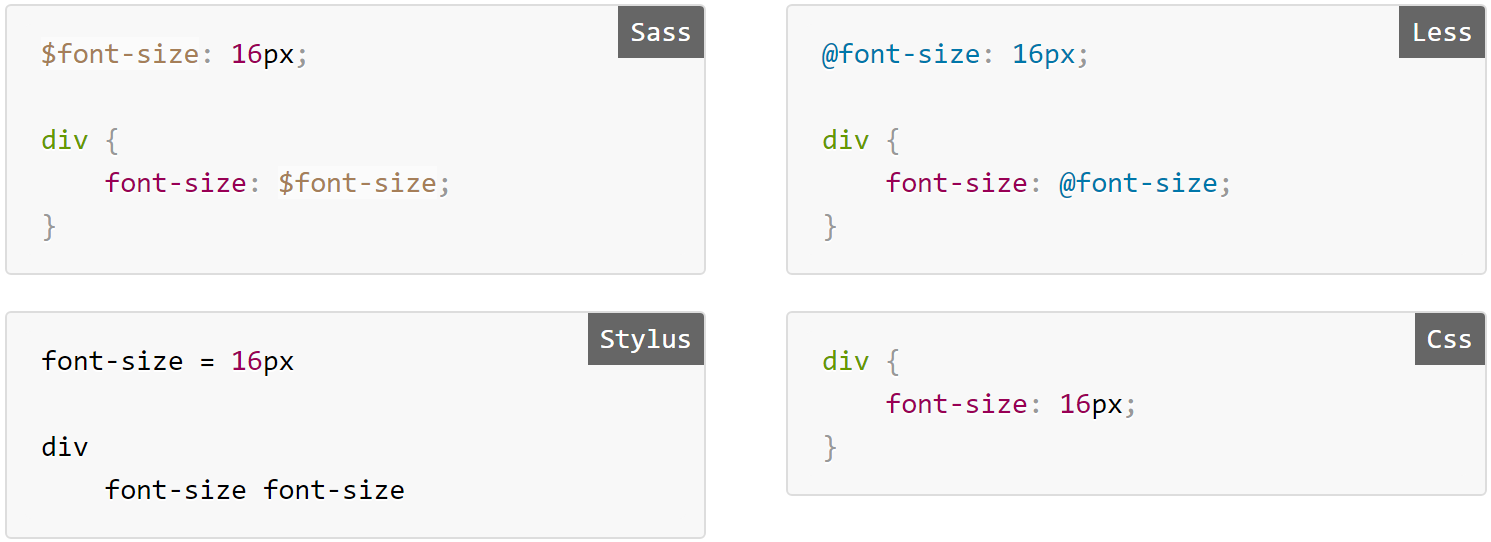
\includegraphics[width=\linewidth]{figs/spm3/css-prepro-variables}
	\caption{Syntax forskelle for brug af variabler.}
	\label{fig:css-prepro-variables}
\end{figure}

\subsubsection{Autoprefixer}
Open-source parser til css, som automagisk tilføjer browserspecifikke prefixes. Som udvikleres skal der nu kun skrives ren CSS. 

\subsection{Build tools}
Bruges til at automatisere opgaver som: minifikation, kompilering, linting og transpilering.

\begin{itemize}
	\item Gulp 
	\item Grunt
\end{itemize}

Gulp bruger \textit{streams}, som er et set af funktioner som en fil går igennem. Derved bliver filen ændret \textit{in-memory} og kun skrives til disk til slut. Grunt opgaver kan ikke blive \textit{chained}.

\subsection{Progressive Web Apps}
Bruger \textit{Service Workers} og kendetegnes ved en række features, som udover at være responsive er:

\begin{multicols}{2}
\begin{itemize}
	\item Connectivity independent
	\item App-like
	\item Discoverable
	\item Re-engageable
	\item Installable
	\item Linkable
\end{itemize}
\end{multicols}

\subsubsection{Service Worker}
Fungerer som en proxy server, idet at alle kald til internettet går gennem disse hvor svar enten hentes fra cache eller internet. Kører i baggrunden og opdaterer data regelmæssigt.

\subsubsection{App shell}
Figur~\ref{fig:app-shell} forskellen på \textit{indhold} og \textit{app shell}. App shell er et minimum af html, css og js, som skal sendes ud til brugeren og caches som det første.

\begin{figure}[H]
	\centering
	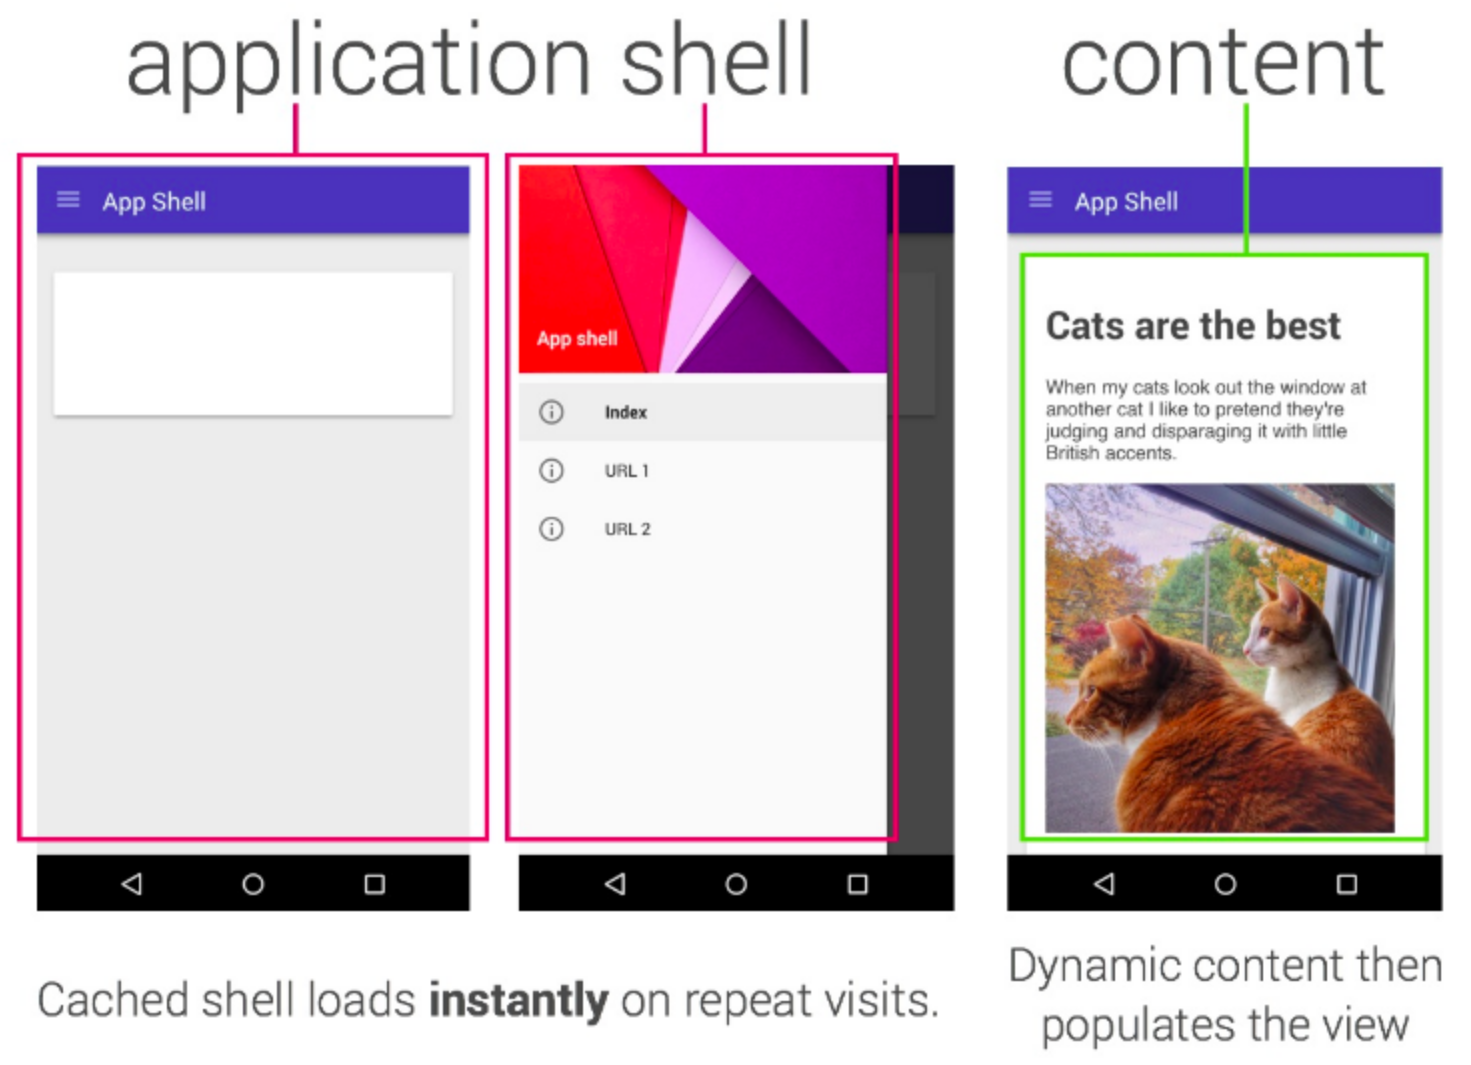
\includegraphics[width=\linewidth]{figs/spm3/app-shell}
	\caption{App shell og indhold.}
	\label{fig:app-shell}
\end{figure}

\subsection{WebSockets og SignalR}
Bruges til 2-vejs kommunikation.

\subsubsection{WebSockets}
